\begin{event}{Atelier PARI/GP 2019b}{AtelierPARI2019b}{Roma (IT),
2018-04-09 to 2018-04-10}{UB}{36}{6}{http://pari.math.u-bordeaux.fr/Events/PARI2019b/}

\textbf{Main goals.} This was a teaching and dissemination meeting, by
invitation from the Roman Number Theory Association as a satellite
event for their 5th mini-symposium.

\textbf{\ODK implication.} \ODK participants: B. Allombert and A. Page from
Bordeaux.

\ODK funded travel and accomodation costs for B. Allombert for about
  1.5k\euro. The ALGANT consortium, LIA LYSM (CNRS) and University Roma Tre
  co-funded the event.

\textbf{Event summary.} This Atelier PARI/GP took place in Roma (Italy) on
April 9th and 10th.  It was followed by a 3-day international research
conference on Number Theory. There were 40 participants for the
Atelier.

The 2-day Atelier followed the same pattern as the previous Roma Atelier
in 2018,
featuring a general introduction to PARI/GP and two
  specialized courses (graduate level) in the mornings:
\begin{itemize}
\item Bill Allombert ``Finite fields'',
\item Aurel Page ``Algebraic number theory''.
\end{itemize}
Afternoons were devoted to practice and problem sessions.

Slides for all talks are available at
\url{http://pari.math.u-bordeaux.fr/Events/PARI2019b/}

\textbf{Results and impact.} This was a successful teaching and dissemination
event, with positive feedback from the participants and organizers.

\begin{figure}[ht]
  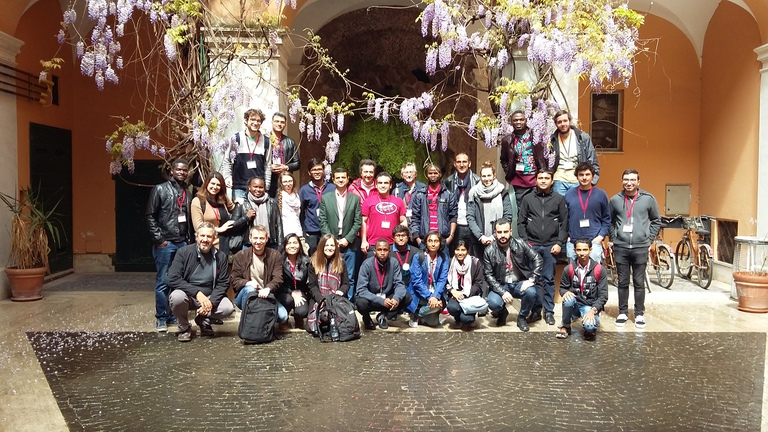
\includegraphics[width=.75\textwidth]{pari2019b.jpg}
  \caption*{Atelier PARI/GP, 5th Roman Number Theory Association mini-symposium, Rome}
\end{figure}
\end{event}
